\begin{figure}[!tbp]
\centering
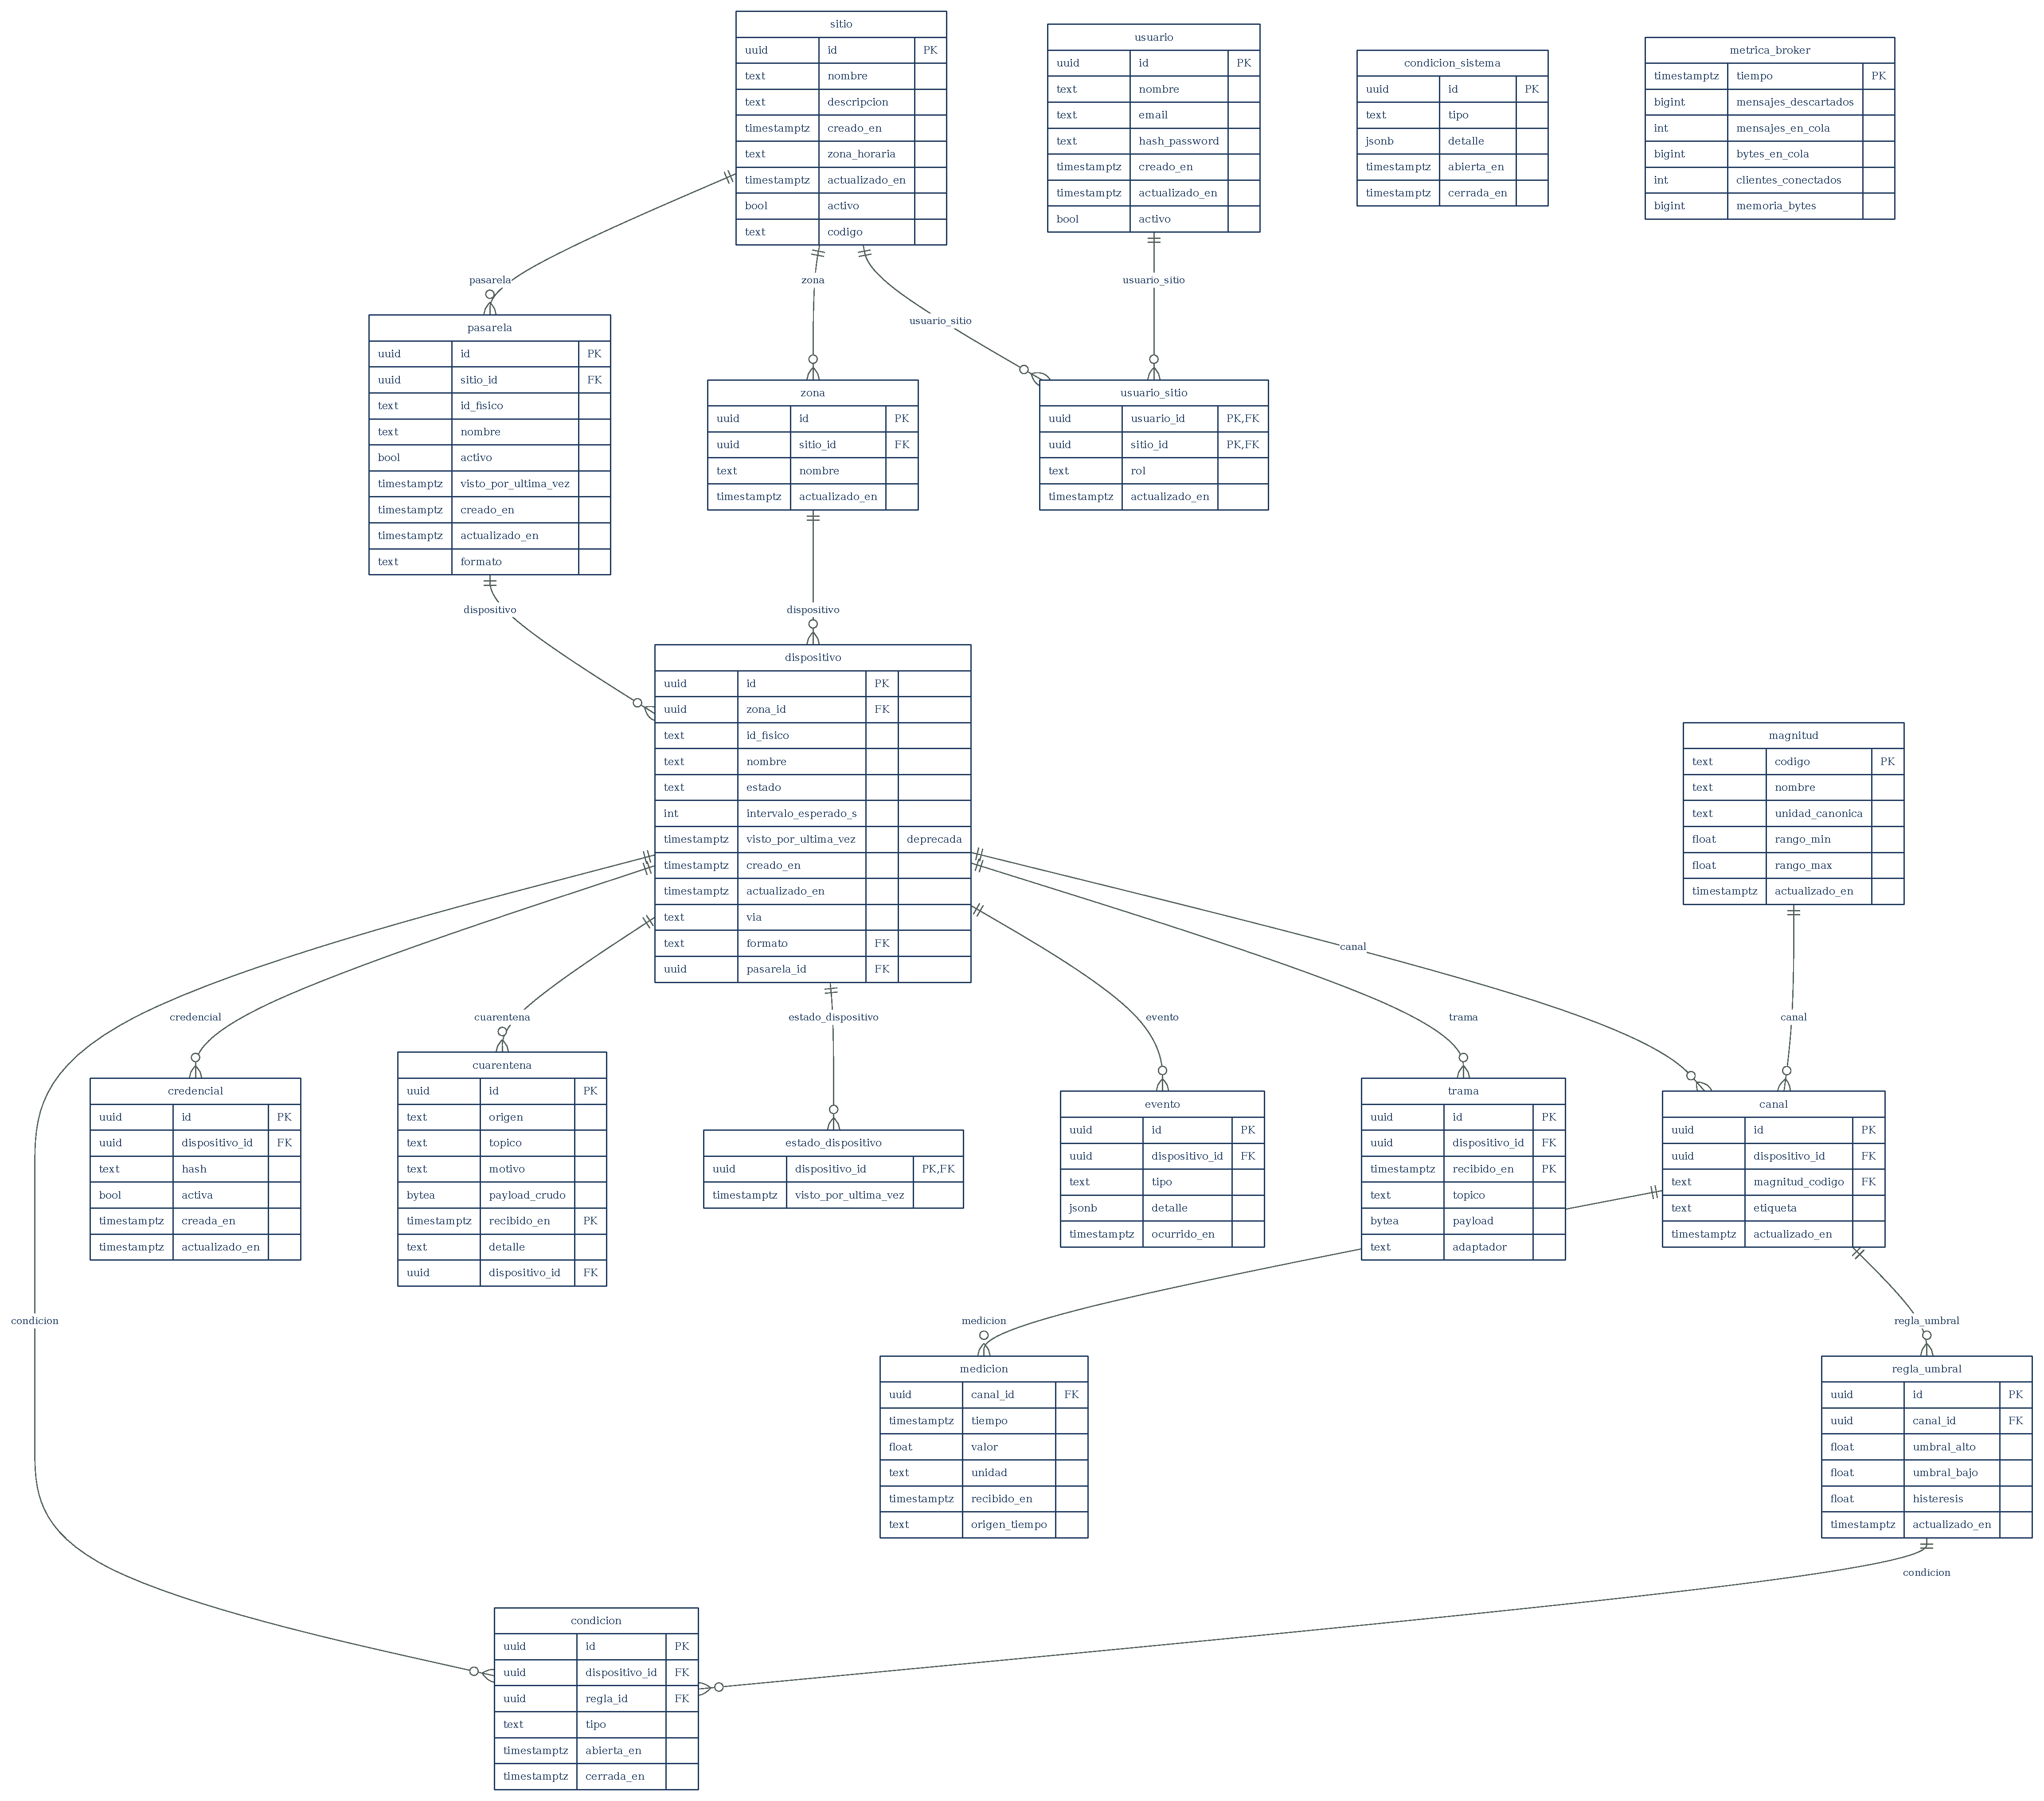
\includegraphics[width=\linewidth,height=0.74\textheight,keepaspectratio]{figuras/render/modelo-datos.pdf}
\caption[Modelo de datos, generado desde el esquema real]{Modelo de datos (diagrama entidad-relación, notación \emph{crow's foot}), generado desde el esquema real de la base de datos. 22 entidades: la organización (\texttt{sitio}, \texttt{zona}, \texttt{usuario} y \texttt{usuario\_sitio}), el acceso de las personas (\texttt{sesion} y \texttt{acceso}), lo propio de cada una (\texttt{preferencia} y \texttt{mensaje\_soporte}), el inventario (\texttt{dispositivo}, \texttt{pasarela}, \texttt{canal}, \texttt{credencial}, \texttt{estado\_dispositivo} y el catálogo \texttt{magnitud}), las series de tiempo (\texttt{medicion}), el estado (\texttt{regla\_umbral}, \texttt{condicion}, \texttt{evento}), lo crudo ---\texttt{trama}, aceptada, y \texttt{cuarentena}, rechazada y atribuida al dispositivo cuando se sabe cuál es--- y la salud del propio sistema (\texttt{condicion\_sistema}, \texttt{metrica\_broker}). \texttt{medicion}, \texttt{trama}, \texttt{cuarentena}, \texttt{metrica\_broker} y \texttt{acceso} son hypertables particionadas por tiempo. Una medición pertenece a un \emph{canal} —dispositivo más magnitud— y no al dispositivo: un nodo que mide temperatura y humedad produce dos series.}
\label{fig:modelo-datos}
\end{figure}
